% nam-csound-icsc.tex — ICSC 2026 submission, llncs template
% blind review: keep AuthorA/AuthorB until camera-ready
% real repo link + acknowledgements go in at camera-ready
\documentclass[runningheads,a4paper]{llncs}

\usepackage{amssymb}
\setcounter{tocdepth}{3}
\usepackage{graphicx}
\usepackage{tikz}
\usetikzlibrary{positioning,arrows.meta}
\usepackage{pgfplots}
\pgfplotsset{compat=1.17}
\usepackage{hyperref}
\usepackage[margin=1.1in]{geometry}
\hypersetup{hidelinks}
\newcommand{\keywords}[1]{\par\addvspace\baselineskip
\noindent\keywordname\enspace\ignorespaces#1}

\pagestyle{headings}

\begin{document}

\mainmatter

\title{Integrating Neural Amp Modeling into Csound}
\titlerunning{Integrating Neural Amp Modeling into Csound}

% TO GUARANTEE THE DOUBLE BLIND REVIEW PROCESS, KEEP GENERIC NAMES
\author{AuthorA\inst{1}\and AuthorB\inst{2} \thanks{Please place acknowledgement here.}}
\authorrunning{AuthorA and AuthorB}
\institute{InstituteA \and InstituteB\\ \email{your.email@yourdomain.com}}

\maketitle

\begin{abstract}
Neural Amp Modeler (NAM) is the most widely used open-source system for
the black-box modeling of nonlinear audio hardware using neural
networks. A community library of several hundred thousand pre-trained
captures exists, but there has been no way to use them inside Csound.
This paper presents \texttt{NAMProcess}, a Csound opcode that performs
real-time NAM inference. The opcode loads standard
\texttt{.nam} model files, switches between models without interrupting audio, adds no algorithmic latency, and runs
comfortably in real time on systems like the Raspberry Pi. A live
dry-referenced volume compensation system built into the opcode holds
every capture in a heterogeneous 25-model test library within $\pm
2$~dB of the player's volume. This paper details the implementation of a thin wrapper around
the NeuralAmpModelerCore C++ library and its integration as a native
plugin opcode, a drag-and-drop Cabbage plugin, and ``tone selection''
in a Raspberry Pi-based guitar pedal.
\keywords{Neural Amp Modeling, Raspberry Pi,
Cabbage Plugin, Opcode, Volume Compensation}
\end{abstract}

\section{Introduction}

Over the past several years a new approach has become standard practice in
guitar audio: record a real device, then train a neural network to
reproduce its input--output behavior. Neural Amp Modeler
(NAM)~\cite{atkinson2025slimmable,nam} is the most widely used
open-source implementation of this approach. Its model format has become a
de facto interchange standard with over 350,000 accumulated on TONE3000
alone~\cite{tone3000} covering amplifiers, effect pedals, preamps, and
other outboard hardware, freely downloadable.

\section{Background and Related Work}

Feedforward WaveNet variants and recurrent LSTM networks are the
established black-box models of guitar amplifiers and distortion
circuits, and both run in real
time~\cite{damskagg2019tube,damskagg2019distortion,wright2019rnn,wright2020realtime,wright2020perceptual}.
NAM~\cite{atkinson2025slimmable,nam} packages both architectures behind
a single model format and a training pipeline whose input is a fixed
published reference signal reamped through the target device.

Real-time inference of such models already exists in the other major
environments. RTNeural~\cite{chowdhury2021rtneural} is a general
inference library for audio callbacks, with a SuperCollider UGen and
Max/MSP and Pure Data ports~\cite{pluta_rtneural}. The
\texttt{neural\_tilde} external loads \texttt{.nam} files in
Max/MSP~\cite{neuraltilde}, \texttt{neural-amp-modeler-lv2} embeds the
NAM core in an LV2 plugin~\cite{oliphantlv2}, and anira treats
real-time-safe inference in audio callbacks
generally~\cite{ackva2024anira}. Csound~\cite{lazzarini2016csound} has
no equivalent. Its prior guitar-gear modeling derives from circuit
knowledge rather than data, like the component-level triode stage opcode of
Fink and Rabenstein~\cite{fink2011triode} or the DSP model of the
Ibanez Tube Screamer pedal series~\cite{walsh2019tubescreamer}. \texttt{NAMProcess} closes that gap.

\section{The NAMProcess Opcode}
\label{sec:opcode}

\subsection{Interface}
\label{sec:interface}

\begin{verbatim}
aoutL, aoutR NAMProcess ainL, ainR,
      kProfileIdx, SLibDir
      [, kAutoVol, kDriveDb]
icount       NAMCount
\end{verbatim}

\texttt{SLibDir} points at a folder, scanned recursively for
\texttt{.nam} files at init. The sorted file list gives every model a
stable index, and \texttt{kProfileIdx} picks one at k-rate. Writing a
new index kicks off an asynchronous load; the running model keeps
playing until the new one is actually ready. \texttt{NAMCount} reports
the library size so orchestra logic can wrap or clamp. Since model
choice is just another k-rate value, tone selection is open to the same
rule-based and generative processes as everything else in Csound,
selection procedures in the sense Koenig
practiced~\cite{koenig1970project2}, not just manual preset browsing.
\texttt{kAutoVol} enables the volume compensation of
Section~\ref{sec:volume}, on by default. \texttt{kDriveDb} is a
pre-model gain in dB whose loudness cost the compensation absorbs,
which turns it into a pure saturation control. A minimal live
instrument:

\begin{verbatim}
instr 1
  aL, aR  ins
  kIdx    chnget "model" ; MIDI, OSC, score
  aoL,aoR NAMProcess aL, aR, kIdx,
          "/home/user/models"
  outs aoL, aoR
endin
\end{verbatim}

Until the first model loads, or if the folder holds no models, audio
passes through untouched. A misconfigured path degrades to bypass, not
silence.

\subsection{Loader and Model State}
\label{sec:loader}

Everything that touches files or network weights runs on a background
thread owned by the opcode, standard real-time audio
discipline~\cite{bencina2011realtime}. The audio thread never
allocates, parses JSON, or blocks on I/O; per k-cycle it takes one
uncontended mutex acquisition to copy a pointer to the active model
pair. The loader builds the requested model, picks the full-quality
submodel for slimmable models~\cite{atkinson2025slimmable}, and
pre-warms internal buffers before publishing the swap. A failed load
keeps the previous model running, so a corrupt file cannot interrupt a
performance; swaps land exactly on a block boundary, click-free.

A model trained at a different sample rate than the engine gets wrapped
in a Lanczos resampling container (the same mechanism the reference
plugin uses) so the network always runs at its trained rate. A 48~kHz
model under a 44.1~kHz engine matches the matched-rate reference within
0.3~dB; without the wrapper the learned filtering stretches by the rate
ratio and the voicing audibly shifts.

NAM models are stateful: WaveNet layers keep convolution history in
ring buffers, LSTMs carry hidden state between calls. So
\texttt{NAMProcess} loads two independent instances of the same file,
resets both off-thread, and publishes them as a pair, one per channel.
That costs an extra load per switch and doubles the model memory, and
it buys exact channel isolation: run both channels through one shared
instance and every block gets convolved against the other channel's
immediate past, which measures as $-4.7$~dB crosstalk on decorrelated
stereo material.

One registration detail worth passing on to other opcode
developers~\cite{lazzarini2017cpof}: registered the conventional way
for an audio-rate generator, \texttt{OENTRY} with \texttt{thread = 5},
the a-rate callback never gets scheduled under Csound 6.18's plugin
path and the opcode emits silence with no error. What works is
\texttt{thread = 3}, computing the whole \texttt{ksmps} block inside
the k-rate callback; declaring \texttt{outypes = "aa"} still allocates
the a-rate outputs.

\subsection{Latency}
\label{sec:latency}

The supported architectures are causal, so the opcode itself should add
no delay, and offline impulse renders agree: response onset lands
within one sample of the input impulse. The only latency left is the
\texttt{ksmps} block granularity every Csound opcode shares, 128
samples or 2.7~ms at 48~kHz in the pedal deployment of
Section~\ref{sec:pedal}.

\section{Live Volume Compensation}
\label{sec:volume}

The opcode continuously matches the wet output to the perceived loudness
of the player's dry signal, so loading any capture (clean, cranked,
mislabeled) leaves the volume unchanged.

Without this, browsing a community library is unusable live: fed the
same signal, the 25 representative captures of Fig.~\ref{fig:bench}
span 17~dB even after a load-time normalization probe, and embedded
loudness metadata does not predict the ranking. No pre-computed
correction can close the gap, because saturating models compress: one
compression-dominated capture holds its output within 1~dB across a
14~dB input sweep, so no per-model gain equalizes it at all. The
correction has to be relative to what the player is actually doing,
and it has to be live.

\begin{figure}
\centering
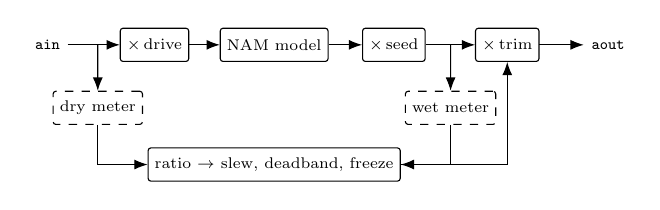
\begin{tikzpicture}[scale=0.8, transform shape,
  box/.style={draw, rounded corners=1pt, minimum height=1.5em,
              inner sep=3pt, font=\scriptsize},
  lbl/.style={font=\scriptsize\ttfamily}, >=Latex]
\node[lbl] (in)    at (0,0)    {ain};
\node[box] (drive) at (1.7,0)  {$\times$\,drive};
\node[box] (model) at (3.6,0)  {NAM model};
\node[box] (seed)  at (5.5,0)  {$\times$\,seed};
\node[box] (trim)  at (7.3,0)  {$\times$\,trim};
\node[lbl] (out)   at (8.9,0)  {aout};
\node[box,dashed] (dm) at (0.8,-1.0) {dry meter};
\node[box,dashed] (wm) at (6.4,-1.0) {wet meter};
\node[box] (ctl) at (3.6,-1.9) {ratio $\rightarrow$ slew, deadband, freeze};
\draw[->] (in) -- (drive);
\draw[->] (drive) -- (model);
\draw[->] (model) -- (seed);
\draw[->] (seed) -- (trim);
\draw[->] (trim) -- (out);
\draw[->] (0.8,0) -- (dm);
\draw[->] (6.4,0) -- (wm);
\draw[->] (dm) |- (ctl);
\draw[->] (wm) |- (ctl);
\draw[->] (ctl) -| (trim);
\end{tikzpicture}
\caption{Live compensation topology inside one \texttt{NAMProcess}
cycle. The dry meter taps the raw input before the drive stage; the
wet meter taps after the model but before the trim.}
\label{fig:comp}
\end{figure}

Dry input and wet output are metered as ITU-R BS.1770 K-weighted mean
squares averaged with a 2.5~s time constant, and a slow output trim tracks
their ratio (Fig.~\ref{fig:comp}). Neither meter observes the trim's
own effect, so the control loop is feed-forward and cannot oscillate. Program dynamics move both meters together and leave the
ratio untouched, so the mechanism is not a compressor. The result is an engineered perceptual invariance: loudness held
constant while spectrum and saturation move. Measured after convergence, a $-12$~dB input step passes through as $-10.2$~dB of output,
the residual being the amp's own compression. The trim engages after one
second of active signal, slews at most 2~dB/s, holds within a 0.75~dB
deadband, freezes below $-55$~dBFS input, and is clamped to $\pm 18$~dB.
Converged trims are remembered per model file: returning to a played
capture lands at level immediately ($+0.6$~dB measured). A load-time
probe seeds the trim for unseen models; the live loop owns the result.

\begin{figure}
\centering
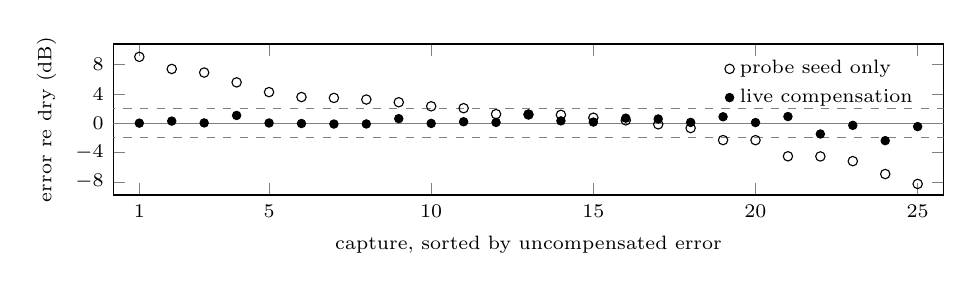
\begin{tikzpicture}
\begin{axis}[width=\linewidth, height=3.5cm,
  xmin=0.2, xmax=25.8, ymin=-9.8, ymax=10.8,
  xlabel={capture, sorted by uncompensated error},
  ylabel={error re dry (dB)},
  label style={font=\scriptsize}, tick label style={font=\scriptsize},
  legend style={font=\scriptsize, draw=none, fill=none,
                at={(0.98,0.97)}, anchor=north east},
  legend cell align=left,
  xtick={1,5,10,15,20,25}, ytick={-8,-4,0,4,8}]
\addplot[gray, thin, domain=0:26, samples=2] {0};
\addplot[gray, thin, dashed, domain=0:26, samples=2] {2};
\addplot[gray, thin, dashed, domain=0:26, samples=2] {-2};
\addplot[only marks, mark=o, mark size=1.7] coordinates {(1,9.04) (2,7.39) (3,6.90) (4,5.56) (5,4.23) (6,3.56) (7,3.44) (8,3.22) (9,2.85) (10,2.30) (11,2.04) (12,1.23) (13,1.18) (14,1.13) (15,0.74) (16,0.38) (17,-0.16) (18,-0.67) (19,-2.31) (20,-2.32) (21,-4.52) (22,-4.54) (23,-5.18) (24,-6.94) (25,-8.29)};
\addplot[only marks, mark=*, mark size=1.5] coordinates {(1,0.00) (2,0.28) (3,0.03) (4,1.05) (5,0.02) (6,-0.05) (7,-0.12) (8,-0.11) (9,0.61) (10,-0.04) (11,0.19) (12,0.10) (13,1.20) (14,0.31) (15,0.15) (16,0.68) (17,0.57) (18,0.10) (19,0.87) (20,0.08) (21,0.90) (22,-1.48) (23,-0.30) (24,-2.39) (25,-0.47)};
\legend{,,,probe seed only,live compensation}
\end{axis}
\end{tikzpicture}
\caption{Loudness error relative to the dry input, all 25 captures on
identical material (saw plucks; peak 300~ms RMS, settled), sorted by
uncompensated error. Dashed lines: $\pm 2$~dB.}
\label{fig:bench}
\end{figure}

Because the dry reference is tapped before the input stage,
\texttt{kDriveDb} pushes the model into saturation without a level change.
$+18$~dB of drive measured $+0.1$~dB of loudness and $-4.6$~dB of crest
factor. Figure~\ref{fig:bench} measures the shipped system: the live loop
collapses the 17.3~dB seed-only spread (standard deviation 4.3~dB) to
3.6~dB (0.74~dB), all but one capture within $\pm 2$~dB of the dry
signal, including the compression-dominated capture that no input
gain can equalize. On the guitar material used during development the
corresponding spread is 3.1~dB (0.83~dB), every capture inside
$\pm 2$~dB; the best purely static probe evaluated left 9.9~dB
(2.60~dB). The official NAM plugin's normalized
output mode applies a static gain from stored metadata or a fixed target.
To our knowledge no published NAM host performs live dry-referenced
compensation.

\section{A Drag-and-Drop Cabbage Plugin}
\label{sec:plugin}

We package the opcode as a VST3/AU plugin through
Cabbage~\cite{walsh2011cabbage}, both as a usable tool and as an
open-source platform for NAM development in Csound. The plugin window is a single drop target: Cabbage publishes the
dropped file's path on its reserved \texttt{LAST\_FILE\_DROPPED}
channel, and a path-input loader variant hot-swaps to it through the
background mechanism of Section~\ref{sec:loader}. The previous amp keeps running until the new one
is ready. Companion opcodes report the actually-loaded model, so
the UI shows real state, and step through the sorted \texttt{.nam}
siblings of the active file for in-folder browsing. The compensation of Section~\ref{sec:volume} defaults on, with an A/B
toggle exposing raw model level. The input control is the drive of
Section~\ref{sec:interface}: saturation, not volume. A gate, three-band tone stack,
and DC blocker mirror the outboard chain of the reference NAM plugin.

The plugin degrades gracefully rather than going silent: an orchestra
that fails to compile emits silence yet passes host validation, so the
base orchestra contains no NAM references and the engine instrument is
compiled at runtime with \texttt{compilestr}. If
the opcode library fails to load, audio passes through dry and the failure
is reported on the status display.

\section{Tone Selection in a Raspberry Pi Guitar Pedal}
\label{sec:pedal}

The opcode's original deployment target is a Raspberry Pi 5-based
guitar pedal running Csound 6.18 at 48~kHz with \texttt{ksmps} 128, the
audio chain pinned to a dedicated core, where the 25-capture library
acts as a bank of ``tones''. Model selection is mapped to MIDI foot
controls and OSC as the k-rate index of Section~\ref{sec:interface}. Because loading is asynchronous and
click-safe the player steps between amps mid-phrase, and because
compensation runs inside the opcode no volume ride accompanies a tone
change. The only added latency is the block granularity
of Section~\ref{sec:latency} (2.7~ms), well inside a live monitoring
budget.
CPU load with a full-quality WaveNet-family model has been informally
observed around 15\% of the audio core during performance.

\section{Conclusions}
\label{sec:conclusions}

\texttt{NAMProcess} gives Csound direct access to NAM's model format
and community library as a drop-in nonlinear processor addressable by a
k-rate index, shipping as a Cabbage plugin and as the tone section of a
Raspberry Pi pedal.

Only one \texttt{NAMProcess} instance per orchestra is currently
supported; lifting this is planned, with an n-channel variant,
persistent trim memory, and Csound 7 plugin support. Source code and measurement tooling
will be released under an open-source license upon publication; the
repository link is omitted to preserve anonymity.

\begin{thebibliography}{22}

\bibitem{ackva2024anira} Ackva, V., Schulz, F.: anira: An Architecture
for Neural Network Inference in Real-Time Audio Applications. In:
Proceedings of the 5th IEEE International Symposium on the Internet of
Sounds (IS2) (2024)

\bibitem{atkinson2025slimmable} Atkinson, S.: Slimmable NAM: Neural Amp
Models with Adjustable Runtime Computational Cost. arXiv:2511.07470 (2025)

\bibitem{nam} Atkinson, S.: Neural Amp Modeler and NeuralAmpModelerCore,
\url{https://www.neuralampmodeler.com},
\url{https://github.com/sdatkinson/NeuralAmpModelerCore}

\bibitem{bencina2011realtime} Bencina, R.: Real-time Audio Programming
101: Time Waits for Nothing,
\url{http://www.rossbencina.com/code/real-time-audio-programming-101-time-waits-for-nothing}

\bibitem{chowdhury2021rtneural} Chowdhury, J.: RTNeural: Fast Neural
Inferencing for Real-Time Systems. arXiv:2106.03037 (2021)

\bibitem{damskagg2019tube} Damsk\"agg, E.-P., Juvela, L., Thuillier, E.,
V\"alim\"aki, V.: Deep Learning for Tube Amplifier Emulation. In:
Proceedings of the IEEE International Conference on Acoustics, Speech and
Signal Processing (ICASSP), pp. 471--475. Brighton (2019)

\bibitem{damskagg2019distortion} Damsk\"agg, E.-P., Juvela, L.,
V\"alim\"aki, V.: Real-Time Modeling of Audio Distortion Circuits with
Deep Learning. In: Proceedings of the 16th Sound and Music Computing
Conference (SMC), pp. 332--339. M\'alaga (2019)

\bibitem{fink2011triode} Fink, M., Rabenstein, R.: A Csound Opcode for a
Triode Stage of a Vacuum Tube Amplifier. In: Proceedings of the 14th
International Conference on Digital Audio Effects (DAFx-11), pp. 365--370.
Paris (2011)

\bibitem{koenig1970project2} Koenig, G.M.: Project 2: A Programme for
Musical Composition. Electronic Music Reports 3. Institute of Sonology,
Utrecht State University, Utrecht (1970)

\bibitem{lazzarini2017cpof} Lazzarini, V.: The Csound Plugin Opcode
Framework. In: Proceedings of the 14th Sound and Music Computing
Conference (SMC), pp. 267--274. Espoo (2017)

\bibitem{lazzarini2016csound} Lazzarini, V., Yi, S., ffitch, J., Heintz,
J., Brandtsegg, {\O}., McCurdy, I.: Csound: A Sound and Music Computing
System. Springer, Cham (2016)

\bibitem{oliphantlv2} Oliphant, M.: neural-amp-modeler-lv2,
\url{https://github.com/mikeoliphant/neural-amp-modeler-lv2}

\bibitem{pluta_rtneural} Pluta, S.: RTNeural Real-Time Neural Inference
UGen, \url{https://scsynth.org/t/rtneural-real-time-neural-inference-ugen/10074}

\bibitem{neuraltilde} Presta, A.: neural\_tilde: Neural Amp Modeler
External for Max/MSP, \url{https://github.com/apresta/neural_tilde}

\bibitem{tone3000} TONE3000, \url{https://www.tone3000.com}

\bibitem{walsh2011cabbage} Walsh, R.: Developing Csound Plugins with
Cabbage. In: J. Heintz, A. Hofmann, I. McCurdy (eds.) Ways Ahead:
Proceedings of the First International Csound Conference. Cambridge
Scholars Publishing, Newcastle upon Tyne (2013)

\bibitem{walsh2019tubescreamer} Walsh, R., Walsh, C.: Digital Signal
Processing Techniques Used to Model the Ibanez Tube Screamer Guitar
Pedal. In: Proceedings of the 5th International Csound Conference
(ICSC 2019). Cagli (2019)

\bibitem{wright2019rnn} Wright, A., Damsk\"agg, E.-P., V\"alim\"aki, V.:
Real-Time Black-Box Modelling with Recurrent Neural Networks. In:
Proceedings of the 22nd International Conference on Digital Audio Effects
(DAFx-19), pp. 173--180. Birmingham (2019)

\bibitem{wright2020realtime} Wright, A., Damsk\"agg, E.-P., Juvela, L.,
V\"alim\"aki, V.: Real-Time Guitar Amplifier Emulation with Deep
Learning. Applied Sciences 10(3), 766 (2020)

\bibitem{wright2020perceptual} Wright, A., V\"alim\"aki, V.: Perceptual
Loss Function for Neural Modelling of Audio Systems. In: Proceedings of
the IEEE International Conference on Acoustics, Speech and Signal
Processing (ICASSP), pp. 251--255. Barcelona (2020)

\end{thebibliography}

\end{document}
